\newpage
\subsection{convert}

\subsubsection{TOF $\rightarrow m/q$}

\subsubsection{Signal labeling - single coincidence}
By repeating a certain filtering operation onto the same signal, but with changing filtering conditions, an array with a set of labels can be written. In this example we only discuss the labeling of TOF hits to `Mass-over-charge' values.\\
For example: A TOF between 950 and 1000 ns is understood as hits that originate from a mass2charge value of 1, and a TOF between 4080 and 4120 ns is understood to come form a mass2charge value of 18. A label array contains expected mass2charge values at the corresponding hits that are identified to belong to that mass2charge. There will be broadening of any TOF peak, but we can label all peaks around a certain expectation value. This broadening is called the `search radius' in this code. Signal labeling can be done for an array of expected mass2charge values, resulting in an array with a label for every hit. No identification of a hit will result in NaN. \\
The definition of the conversion factor is as follows:
\begin{equation}
TOF = t_0 + factor*\sqrt(M2Q)
\end{equation}
Note that the $t_0$ is a correction value and is already substracted from the measured TOF in the `correct' section.

\subsubsection{Signal labeling - double coincidence}
In the case of a double coincidence event (two hits registered on one detector in one event), the filtering conditions of the measurement can be fine tuned. In this software, two methods are available;  the `circle', in which a certain maximum distance between the nominal m2q-values are approved. The other method, `line', approves all hits along a diagonal line representing a constant TOF. 

\paragraph{circle} In a two-dimensional histogram of two mass-over-charge values, only hits within a certain circle are approved. This can be of use in the case of cluster measurements, where the momenta of two cations are not necessarily related. See Figure \ref{labeling_C2} for an example.

\begin{figure}[H]
   \centering
    \centerline{\includegraphics[width=0.9\textwidth]{Graphics/M2Q_labeling_C2_circle_example.eps}}
\caption{example of a `circle' filter around the nominal mass-over-charge values. Circle radius of 0.25 mass-over-charge units. Example of water-ammonia clusters.}
\label{labeling_C2}
\end{figure}

\paragraph{line} 
In a two-dimensional histogram of two mass-over-charge values, only hits with a TOF-sum that is close to the nominal one, is approved. This is useful when the detection is complete, and can therefore be regarded to have opposite momenta in z-direction. 

\begin{figure}[H]
   \centering
    \centerline{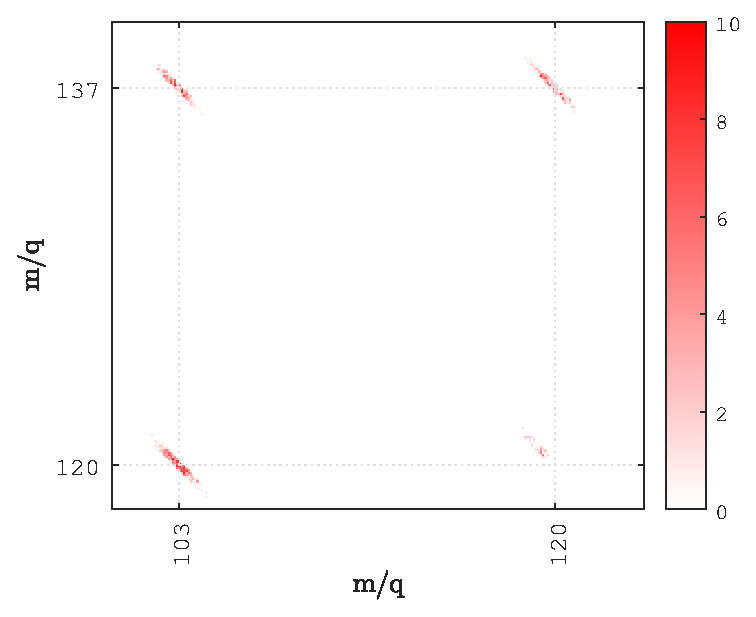
\includegraphics[width=0.5\textwidth]{Graphics/M2Q_labeling_C2_line_example.eps}}
\caption{Example of a `line' filter around the nominal mass-over-charge values. Circle radius of 0.2 mass-over-charge units. Example of ammonia clusters.}
\label{labeling_C2}
\end{figure}

\subsubsection{Branching ratio's}
The braching ratio is defined here as the relative number of hits registered for a label, or a set of labels. In the presented example, branching ratio's of mass-over-charge labels are shown. \\

\paragraph{Single-label Branching ratio's}

The Branching ratio of single labels simply counts the number of hits are categorized into a certain label. As an example, figure \ref{BR_1D} shows the number of occurences of particles recognized as having certain mass-2-charge values. Note that these labels can be defined independently from the events.

\begin{figure}[H]
   \centering
    \centerline{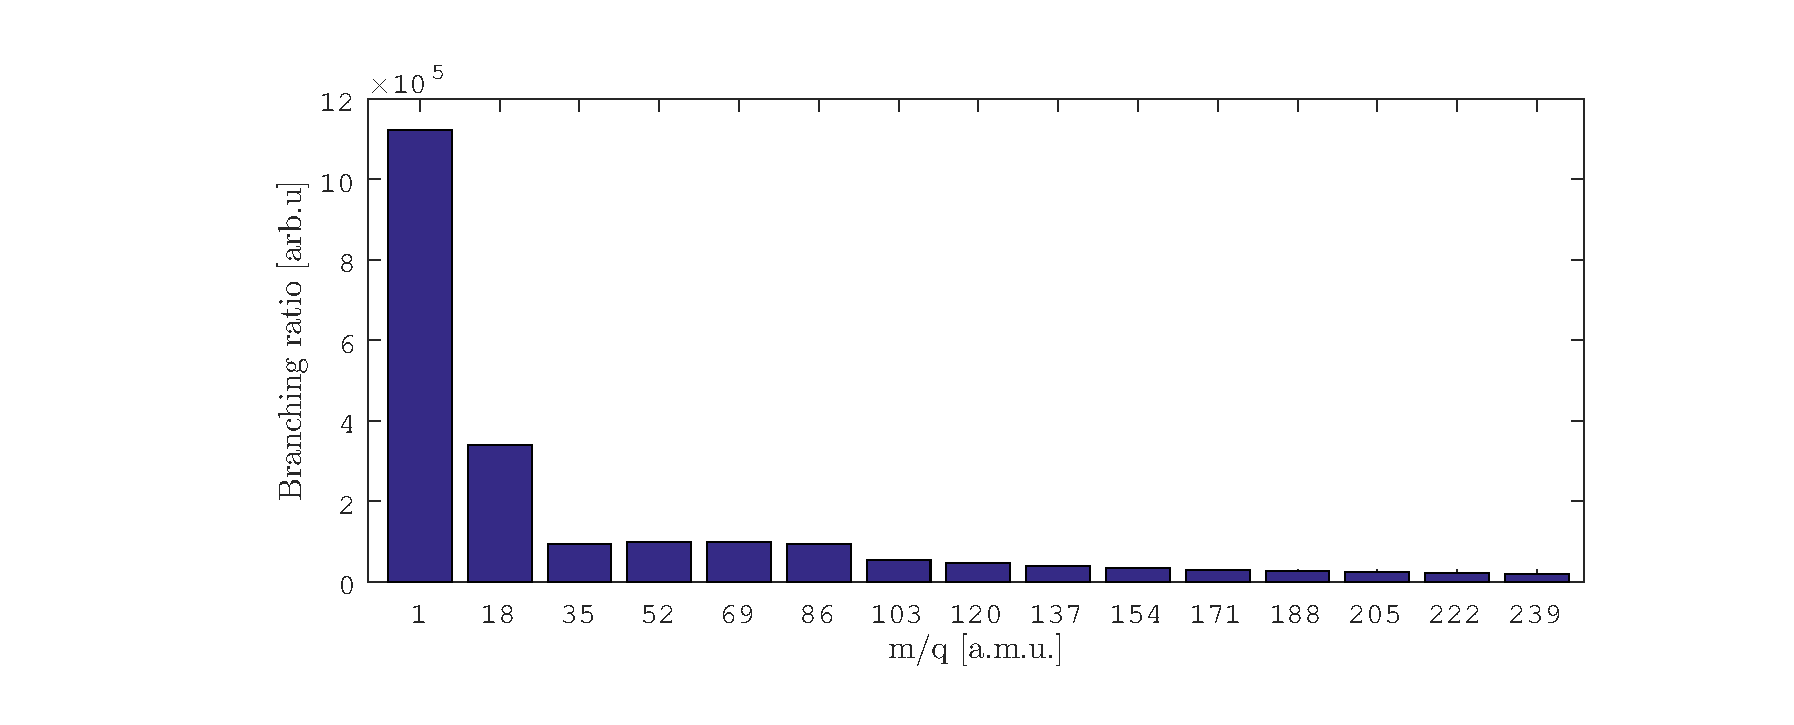
\includegraphics[width=0.9\textwidth]{Graphics/BR_1D.eps}}
\caption{Example of a branching ratio plot. This example: NH$_3$ clusters, filename called `20091115\_NH3\_n17'}
\label{BR_2D}
\end{figure}

\paragraph{Double-label Branching ratio's}
If multiple hits are registered in one event, the possible combinations of labels can be studied. If there are $n$ labels registered, then $n^2$ combinations of labels can be registered. The double-label branching ratio is the histogram of these combinations, with a differentiation between label A registered before label B and label A registered after label B. In Figure \ref{BR_2D}, an example of such two-label branching ratio plot is shown. It shows which mass-to-charge particle is registered in combination with another. All the first labels registered have smaller mass-to-charge values, because the labels are based on the TOF values of the hits.

\begin{figure}[H]
   \centering
    \centerline{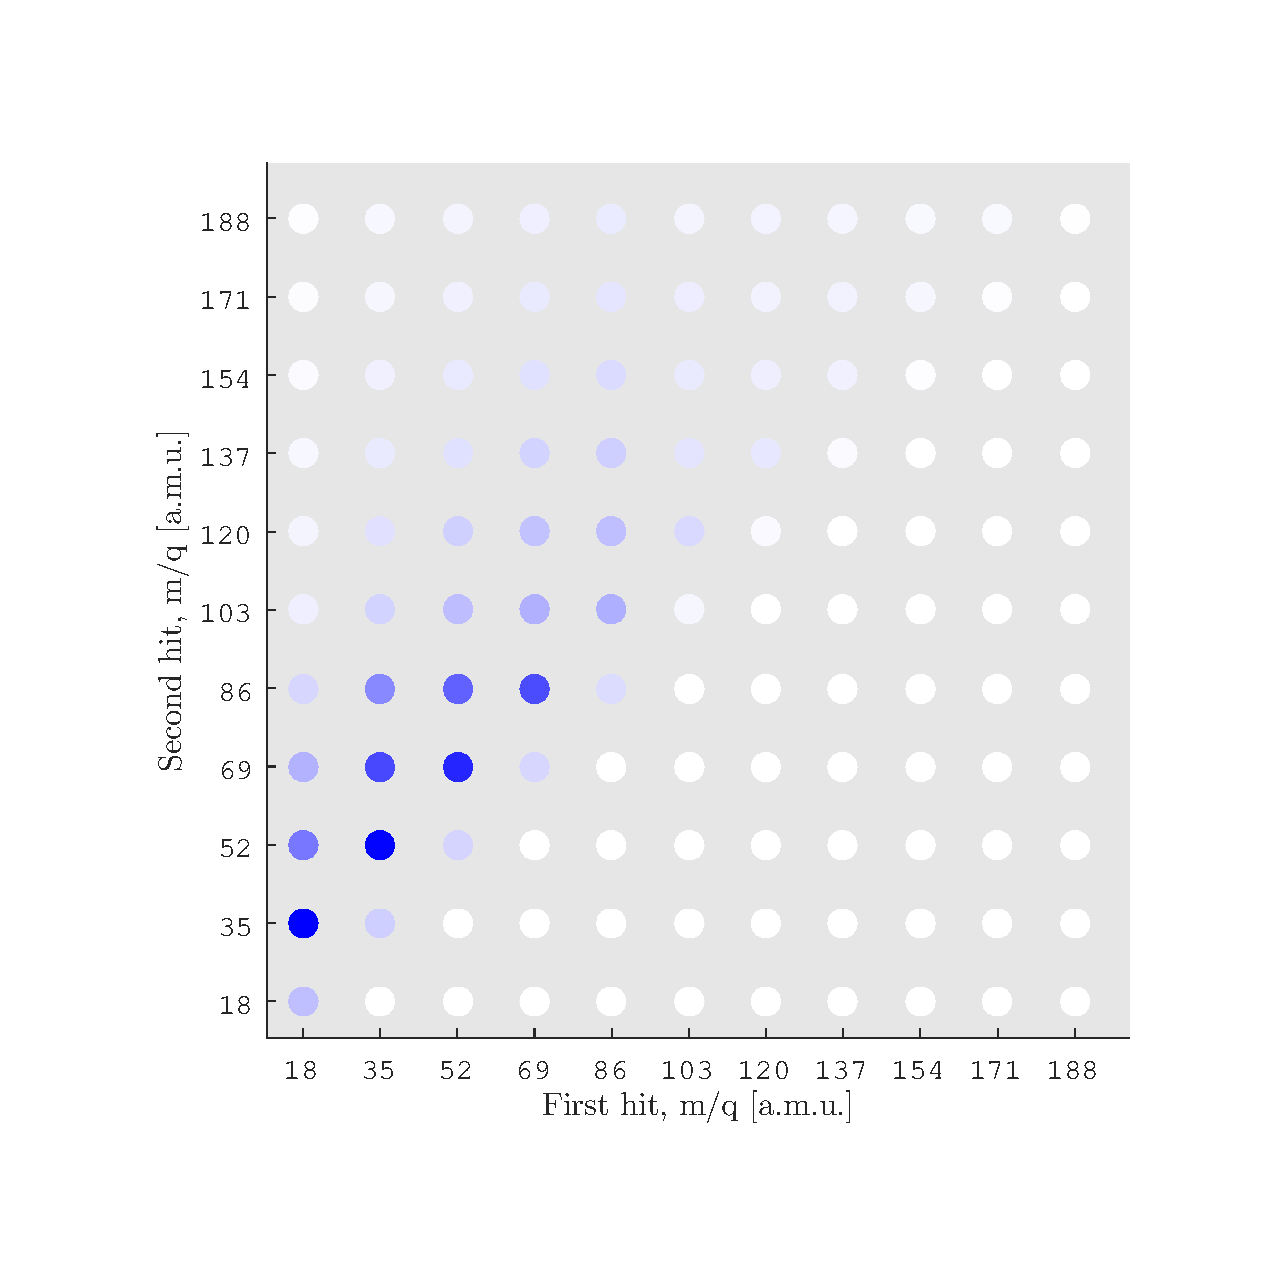
\includegraphics[width=0.6\textwidth]{Graphics/BR_2D.eps}}
\caption{Example of a branching ratio plot for double labels (double coincidence). The color of the dots represents the branching ratio of that set of labels. This example: NH$_3$ clusters, filename called `20091115\_NH3\_n17'}
\label{BR_1D}
\end{figure}

\subsubsection{Momentum}

TODO: describe the Maxwell-Boltzmann distribution assumption!
\begin{align}
V_{avg} = \sqrt{\frac{\gamma}{\gamma - 1}} \sqrt{\frac{2 R T}{W}}
\end{align}

\begin{figure}[H]
  \centering
  \vspace{0 cm}
  \def\svgwidth{200pt}
  \centerline{\input{Graphics/momentum_subtraction.pdf_tex}}
  \caption{Schematic of the Momentum along the molecular beam, $\vec{p}_{0}$}
\end{figure}


In the case of momentum imaging, the splat radius on the detector gives info about the momentum in the transverse direction (here called the $x$ and $y$-direction. In the first approximation, the splat radius increases linearly with the momentum in each direction.\\
The momentum in the detector axis can be inferred from the difference between the actual and the zero kinetic energy time of flight of the particle.\\
The sample, leaving the molecular beam, has a low mean velocity in directions perpendicular to the beam. However, the velocity distribution in the molecular beam direction has a higher mean value. 
This will show up in the data as a spatial shift of the detection centre at higher Times Of Flight. 

\begin{figure}[H]
   \centering
    \centerline{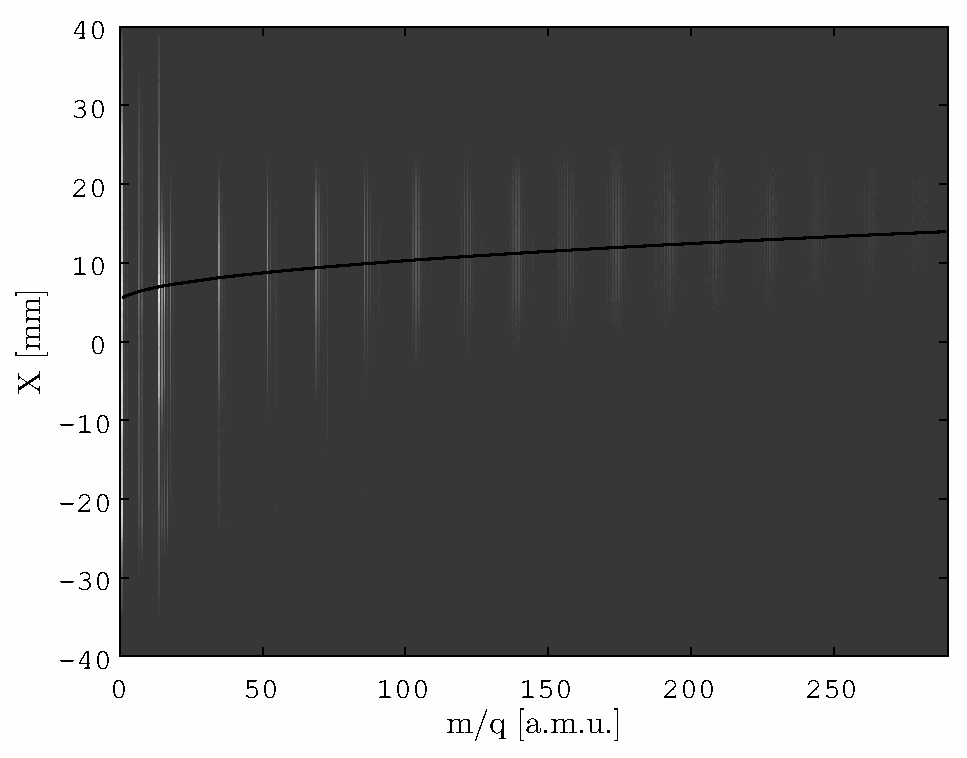
\includegraphics[width=0.9\textwidth]{Graphics/p_0_subtraction_before.eps}}
\caption{Radius vs TOF, showing the shift of hits outward. The line is plotted with a prediction from a Maxwell-Boltzmann expectation value of the velocity ($T_{sample} = $ 38 [deg]). Example: Ammonia/Water clusters at 450 eV. (20130903\_008.dlt)}
\end{figure}

The momentum in x and y-direction (parallel to detector plane) can be calculated from the simple equation $s = v \cdot t$:

\begin{equation}
\vec{p}_{x, y} =  \frac{m \cdot X}{TOF}
\end{equation}

The momentum in z-direction (perpendicular to detector plane) is calculated as:

\begin{equation}
\vec{p}_{z} = q \cdot E_{ER} \cdot \Delta TOF
\label{p_z_2_TOF}
\end{equation}
where $\Delta TOF$ is defined as the difference between the zero-momentum Time Of Flight and the actual Time Of Flight. $E_{IR}$ is the electric field strength in the interaction region.
We define two different momenta: the momentum of the sample before the photon interaction takes place ($\vec{p_0}$), and the momentum after the interaction has taken place ($\vec{p}$). Note that the kinetic energy released following photon interaction should calculate with the difference of these two vectors:

\begin{equation}
KE = KE(\vec{p} - \vec{p_0}) = \frac{1}{2 m} \cdot |{\vec{p} - \vec{p_0}}|^2
\end{equation}

\paragraph{$\vec{p_0}$ determination}
The zero-time momentum $\vec{p_0}$ is determined from the difference in the mean value of the X, Y and TOF and their zero-momentum expectation values. These zero-momentum expectation values are 0 for X and Y (assuming a proper correction of the detection centre, see signal correction), and given by the expected mass over charge labels for the TOF signal. The averaging is done over all hits belonging to one label. For instance, a label could be an OH$^+$ fragment. 

\paragraph{$\vec{p}$ determination}
The final momentum $\vec{p}$ is determined by the difference in measured detector position and the zero-momentum expectation values. Note that this value can be different for every hit, whereas $\vec{p_0}$ is determined for every label (containing multiple hits). 

\begin{figure}[H]
   \centering
    \centerline{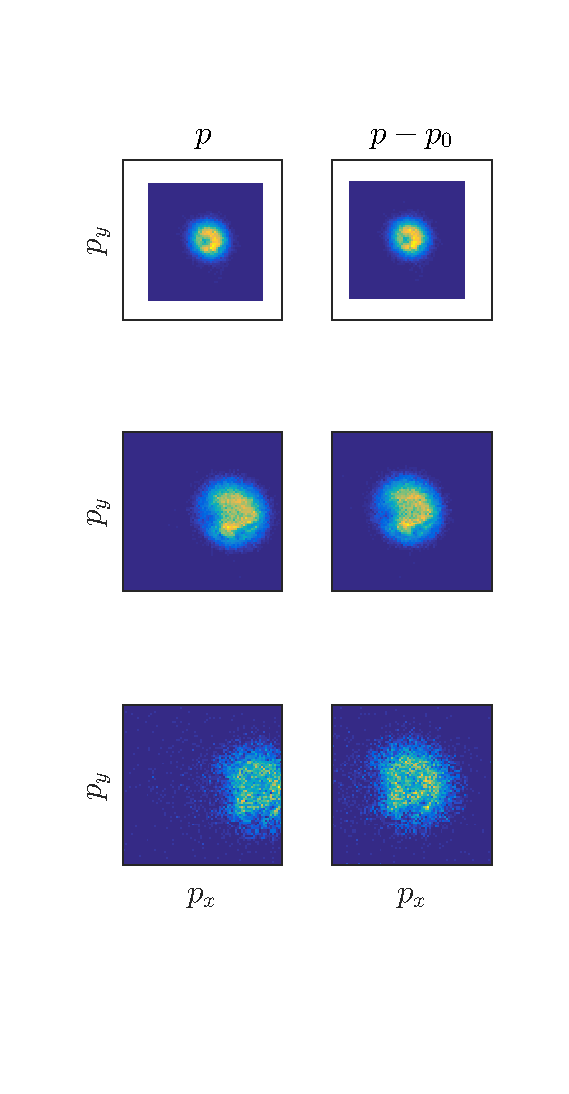
\includegraphics[width=0.4\textwidth]{Graphics/pxpy_hist.eps}}
\caption{The total momentum ($p$) and the total minus the zero-time momentum ($p - p_0$) compared. In this example, the molecular beam is directed along the x-axis, coming from the left. It is seen that the mean value of total momentum shifts along the molecular beam axis, which is  
Example of pure NH3 clusters for cluster sizes of n = 1, 5, 10 in (NH$_3$)$_n^+$H}
\end{figure}

\subsubsection{Kinetic Energy Release}

If all three momentum components of a particle can be determined, the kinetic energy of that particle can be calculated:

\begin{equation}
KE = \frac{1}{2 m} \cdot \left(p_x^2 + p_y^2 + p_z^2 \right)
\end{equation}

\begin{figure}[H]
    \centering
        {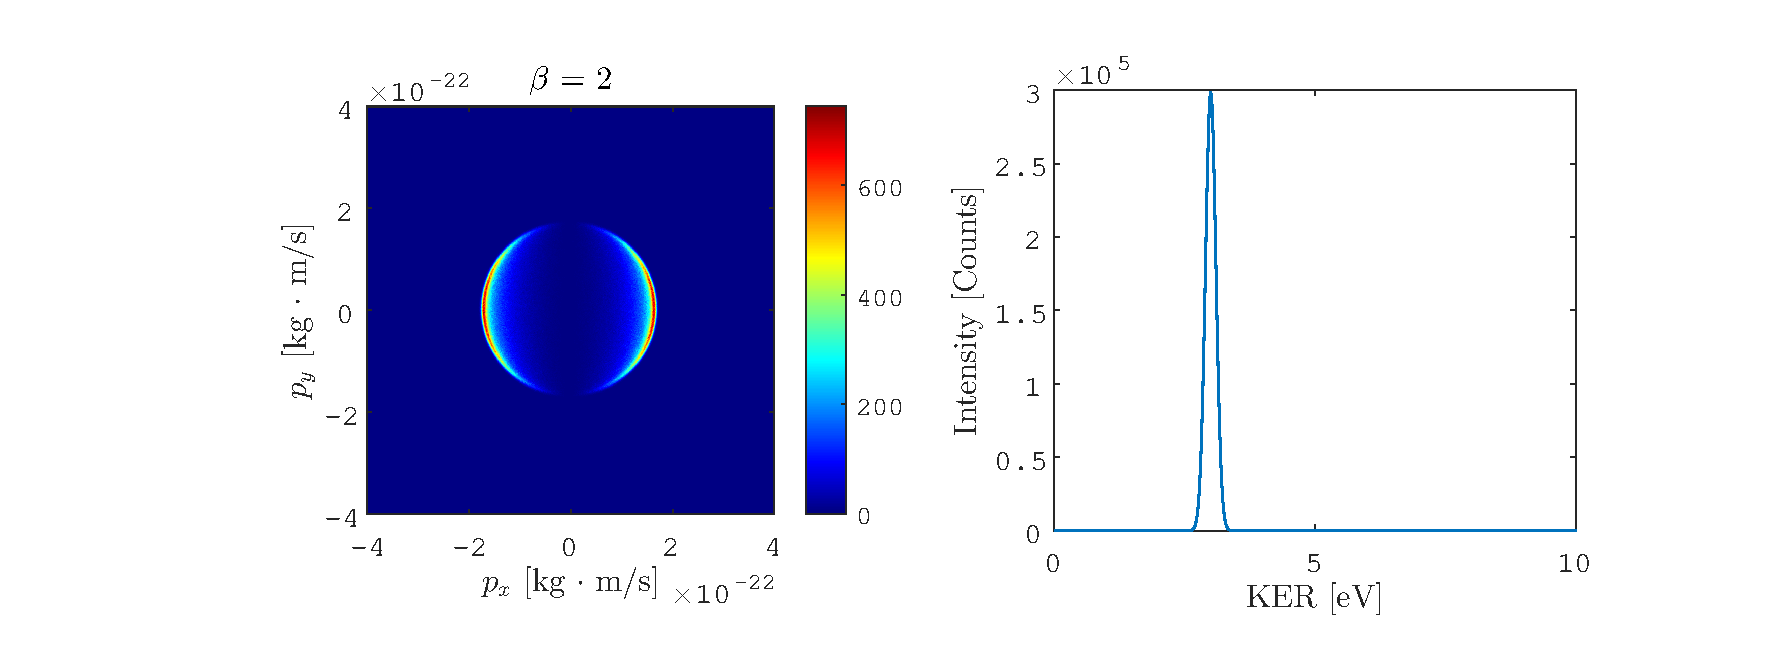
\includegraphics[width=0.7\textwidth]{Graphics/KER_dummy_data_beta_2.eps}
    }\\
        {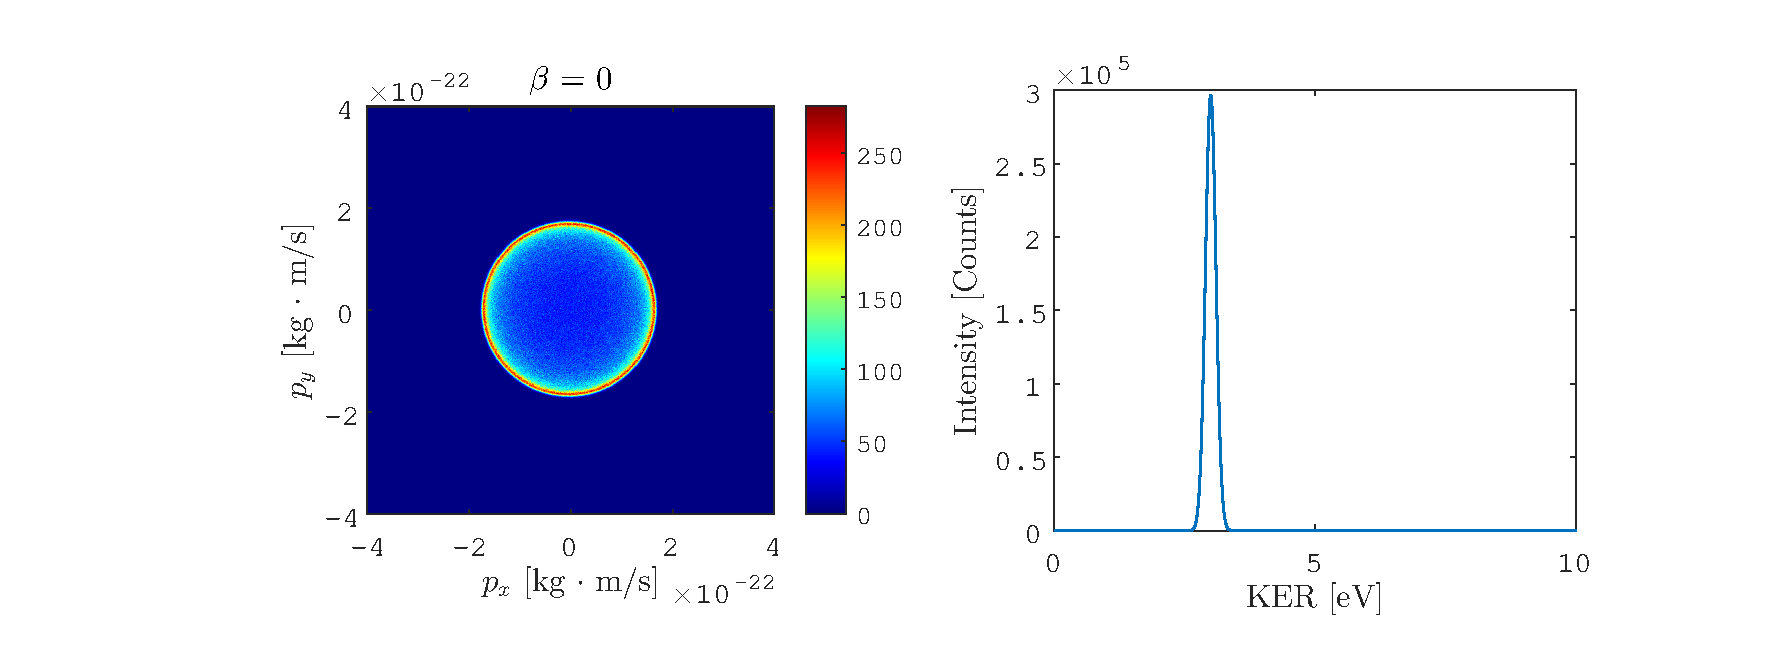
\includegraphics[width=0.7\textwidth]{Graphics/KER_dummy_data_beta_0.eps}
    }\\
        {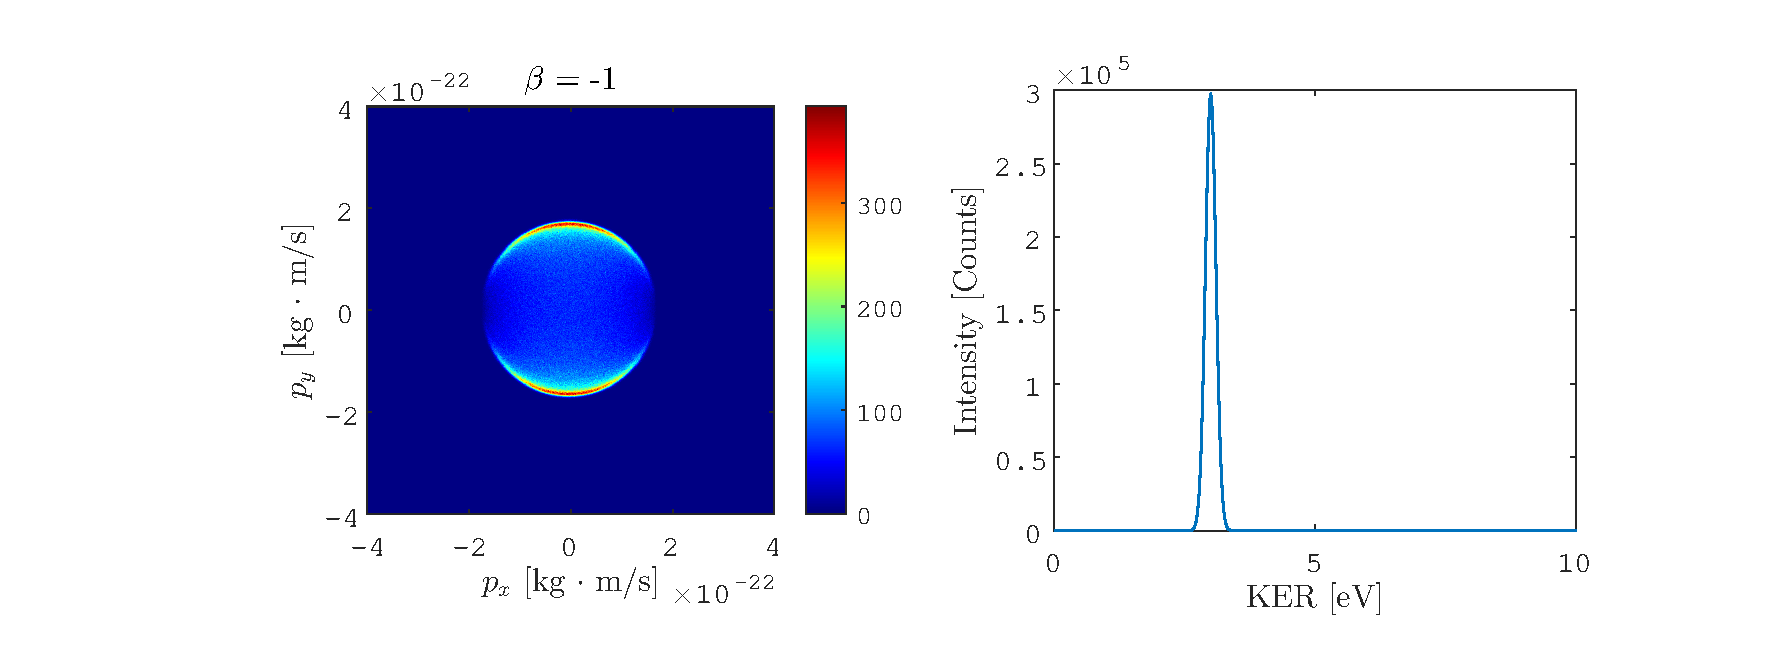
\includegraphics[width=0.7\textwidth]{Graphics/KER_dummy_data_beta_-1.eps}
    }
    \caption{The kinetic energy release does not change for different angular distributions ($\beta$-values). Fake data created with the parameters: m = 18 a.m.u, singly charged, KE = 3 eV, $\sigma$(KE) = 0.1eV. Polarization is horizontal in the screen.}
    \label{TS}
\end{figure}

\subsubsection{Mutual momentum angle}
the angle between two three-dimensional momentum vectors is measured by the shortest great circle path between them, which means that it must lie between 0 and pi radians.

\begin{figure}[H]
  \centering
  \vspace{0 cm}
  \def\svgwidth{200pt}
  \centerline{\input{Graphics/mutual_angles.pdf_tex}}
  \caption{The shortest great circle path between two three-dimensional momentum vectors is called $\theta$.}
\end{figure}

\subsubsection{Asymmetry parameter $\beta$}
TODO

\subsubsection{Interaction point}
In the event of complete ion detection of an initially cold sample, the initial source point position can be calculated. If we assume the sum of all momenta to be equal to zero:

\begin{equation}
p_{res, x} = \sum_i {\frac{m_i \cdot (X_i - X_{0})}{TOF_i}} = 0
\end{equation}
where $i$ is the amount of hits registered in one event. Form this equation, we can extract information on the creation point of the mother particle. This equation can in general be solved for any $i$:

\begin{equation}
X_0 = \frac{ \sum_i {\tfrac{m_i}{TOF_i} X_i} }
						{ \sum_i {\tfrac{m_i}{TOF_i} } }
\label{X_CM}
\end{equation}

In the case of a single-hit event, equation \ref{X_CM} simplifies to $X_0 = X_1$, so in these approximations, the registration of mother ions images the source volume. Equation \ref{X_CM} is valid for X and Y. \\
For the Z-direction (TOF), we identify three contributions to the measured TOF:

\begin{align}
\underbrace{TOF_{exp}} _\textrm{measured TOF} &= 
\underbrace{TOF  (Z = 0, p = 0)}_\textrm{nominal TOF, or $TOF_0$} + 
\underbrace{\Delta TOF (Z = 0, p = p_z)}_\textrm{p-induced TOF shift} +
\underbrace{\Delta TOF (Z = Z_0, p = 0)}_\textrm{Z-induced TOF shift}
\end{align}

The TOF difference induced by the momentum can be written as (see Eq. \ref{p_z_2_TOF}):

\begin{equation}
\Delta TOF (Z = 0, p = p_z) = \frac{p_z}{q \cdot E_{ER}}
\end{equation}

The TOF difference induced by the Z-displacement is the relation under study here. Note that this number is minimized by the Wiley-McLaren condition, so this calculation can be error-prone when exact Wiley-McLaren conditions are met. We assume the linear condition:

\begin{equation}
\Delta TOF (Z = Z_0, p = 0) = \frac{C \cdot Z_0}{\sqrt{m/q}}
\end{equation}

In case of Wiley McLaren conditions met, C = 0 (see Figure \ref{dZ_vs_dTOF_Laksman}), and the presented treatment cannot be used.

\begin{figure}[H]
   \centering
    \centerline{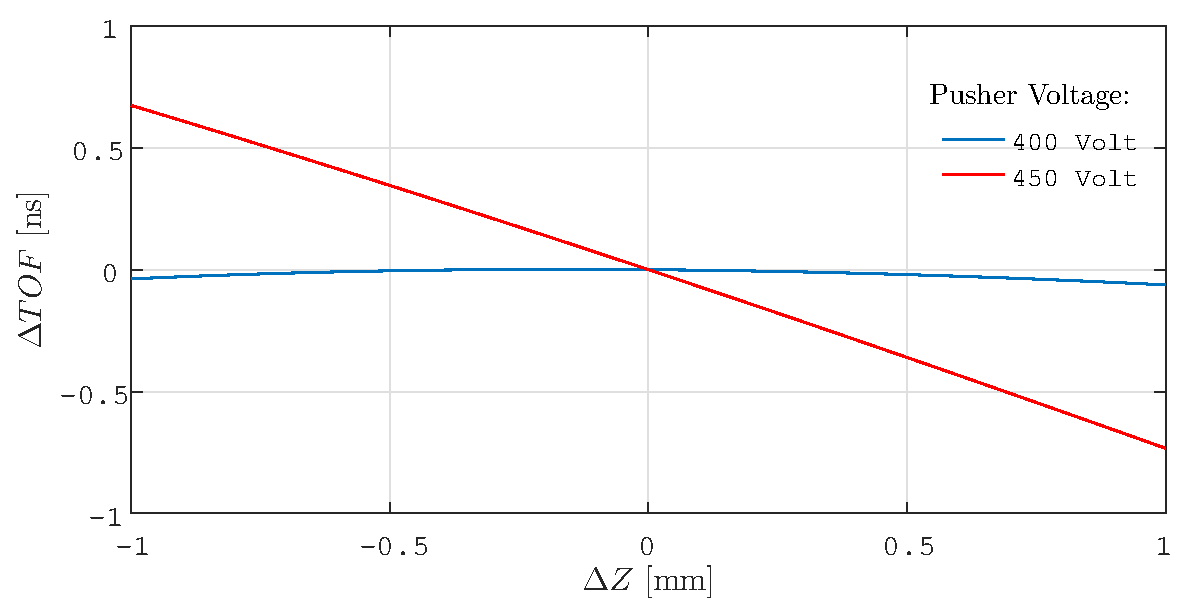
\includegraphics[width=0.8\textwidth]{Graphics/dZ_vs_dTOF_Laksman.eps}}
\caption{Example of how the change in dZ affects the effective (TOF Laksman). Two examples of ion `pusher' voltages are shown. The 400 Volt example meets the Wiley-McLaren condition, but the 450 Volt example does not. In this treatment, the correlation is assumed linear. $m/q = 1$, Drift tube voltage = -4kV.}
\label{dZ_vs_dTOF_Laksman}
\end{figure}

With this description of the TOF, we can use momentum conservation:

\begin{align}
p_{res, z} = \sum_i{p_{z, i}} = E_{ER} \cdot \sum_i{\left( TOF_{exp, i} - TOF_0 - \tfrac{b \cdot Z_0}{\sqrt{m/q_i}} \right) \cdot q_i} = 0\\
\sum_i{\left( TOF_{exp, i} - TOF_0 \right) \cdot q_i} = 
\sum_i{\tfrac{b \cdot Z_0}{\sqrt{m/q_i}} \cdot q_i }
\end{align}

Note that $Z_0$ is an event property, and is thus the same for all hits in the same event. To write $Z_0$ explicitly:

\begin{equation}
Z_0 = \frac{\sum_i{\left( TOF_{exp, i} - TOF_0 \right) \cdot q_i}}
{\sum_i{b \cdot \sqrt{\tfrac{q_i^3}{m}}}}
\end{equation}

Or, more general, not assuming a linear relation between the $\Delta TOF $ and $Z_0$:
\begin{equation}
a + b \cdot Z_0 + c \cdot Z_0^2 + ... = \frac{\sum_i{\left( TOF_{exp, i} - TOF_0 \right) \cdot q_i}}
{\sum_i{\sqrt{\tfrac{q_i^3}{m}}}}
\end{equation}

This conversion is only implemented for X and Y. See `convert.source$\_$position' for the code so far.

\subsubsection{Oversight of signals}

Here, a signal is defined as something that has a value for all hits. New signals are created by correcting a raw signal or converting a corrected signal. The signals can be found in: \emph{`Experiment name'.h.`detector name'}.`signal name'. The momentum is expressed in atomic units. \footnote{($ 1 a.u. = 1.992e-24 \cdot \tfrac{kg \cdot m}{s}$)}	

\begin{tabular}{l|c|c|c|r}
Description & MATLAB name & Type & Created from & Unit\\
\hline
detector dependent 						& raw 							& input	 								& - 														&- \\
corrected X										& X\_corr						& corrected						& X (raw)		 									& mm \\
corrected Y										& Y\_corr						& corrected						& X (raw) 										& mm \\
corrected TOF									& TOF\_corr				& corrected						& TOF(raw)  									& ns \\
mass-to-charge 								& m2q 							& converted 						& TOF\_corr									& $\tfrac{a.m.u}{a.c.u.}$ \\ 
m2q labels											& m2q\_l 					& label 									& m2q												& $\tfrac{a.m.u}{a.c.u.}$ \\ 
mass labels 										& m\_l							& label 									& m2q												& a.m.u \\
zero-time momentum, $\vec{p_0}$			& p\_0		& converted 						& X, Y, TOF, m2q\_l						& a.u.\\
final momentum, $\vec{p}$		& p 									& converted 						& X, Y, TOF, m2q\_l						& a.u.\\
momentum difference, $\vec{p} - \vec{p_0}$ & dp& converted 						& X, Y, TOF, m2q\_l						& a.u.\\
Kinetic energy release 					& KER 							& converted 						& p, p\_0 											& Joule \\
\end{tabular}	


